\documentclass[12pt]{scrartcl}
\usepackage[sexy]{james}
\usepackage[noend]{algpseudocode}
\setlength {\marginparwidth}{2cm}
\usepackage{answers}
\usepackage{array}
\usepackage{tikz}
\newenvironment{allintypewriter}{\ttfamily}{\par}
\usepackage{listings}
\usepackage{xcolor}
\usetikzlibrary{arrows.meta}
\usepackage{color}
\usepackage{mathtools}
\newcommand{\U}{\mathcal{U}}
\newcommand{\E}{\mathbb{E}}
\usetikzlibrary{arrows}
\Newassociation{hint}{hintitem}{all-hints}
\renewcommand{\solutionextension}{out}
\renewenvironment{hintitem}[1]{\item[\bfseries #1.]}{}
\renewcommand{\O}{\mathcal{O}}
\declaretheorem[style=thmbluebox,name={Chinese Remainder Theorem}]{CRT}
\renewcommand{\theCRT}{\Alph{CRT}}
\setlength\parindent{0pt}
\usepackage{sansmath}
\usepackage{pgfplots}

\usetikzlibrary{automata}
\usetikzlibrary{positioning}  %                 ...positioning nodes
\usetikzlibrary{arrows}       %                 ...customizing arrows
\newcommand{\eqdef}{=\vcentcolon}
\newcommand{\tr}{{\rm tr\ }}
\newcommand{\im}{{\rm Im\ }}
\newcommand{\spann}{{\rm span\ }}
\newcommand{\Col}{{\rm Col\ }}
\newcommand{\Row}{{\rm Row\ }}
\newcommand{\dint}{\displaystyle\int}
\newcommand{\dt}{\ {\rm d }t}
\newcommand{\PP}{\mathbb{P}}
\newcommand{\horizontal}{\par\noindent\rule{\textwidth}{0.4pt}}
\usepackage[top=3cm,left=3cm,right=3cm,bottom=3cm]{geometry}
\newcommand{\mref}[3][red]{\hypersetup{linkcolor=#1}\cref{#2}{#3}\hypersetup{linkcolor=blue}}%<<<changed

\tikzset{node distance=4.5cm, % Minimum distance between two nodes. Change if necessary.
         every state/.style={ % Sets the properties for each state
           semithick,
           fill=cyan!40},
         initial text={},     % No label on start arrow
         double distance=4pt, % Adjust appearance of accept states
         every edge/.style={  % Sets the properties for each transition
         draw,
           ->,>=stealth',     % Makes edges directed with bold arrowheads
           auto,
           semithick}}


% Start of document.
\newcommand{\sep}{\hspace*{.5em}}

\pgfplotsset{compat=1.18}
\begin{document}
\title{AMSC460: Homework 3}
\author{James Zhang\thanks{Email: \mailto{jzhang72@terpmail.umd.edu}}}
\date{\today}

\definecolor{dkgreen}{rgb}{0,0.6,0}
\definecolor{gray}{rgb}{0.5,0.5,0.5}
\definecolor{mauve}{rgb}{0.58,0,0.82}

\lstset{frame=tb,
  language=Java,
  aboveskip=3mm,
  belowskip=3mm,
  showstringspaces=false,
  columns=flexible,
  basicstyle={\small\ttfamily},
  numbers=left,
  numberstyle=\tiny\color{gray},
  keywordstyle=\color{blue},
  commentstyle=\color{dkgreen},
  stringstyle=\color{mauve},
  breaklines=true,
  breakatwhitespace=true,
  tabsize=3
}

\maketitle

\begin{proof}[Solution]
  \hfill

  \begin{enumerate}[(a)]
    \item Denote $f = x + \ln x = 0$. $f$ is is continuous and differentiable on the interval on $(0, \infty)$.
    Note that $f(0.1) \approx -2.2$ and $f(1) = 1$. Since $0 \in (-2.2, 1)$, by the Intermediate Value Theorem, 
    $f$ attains all values in between, so $\exists \ x^* \in [0.1, 1]$ such that $f(x^*) = 0$. 
    To show that there is \textit{exactly} one root, assume not and that there are 2 solutions such that 
    \[f(a) = 0 = f(b)\]
    By Rolle's Theorem, $\exists \ c \in (a,b)$ such that $f'(c) = 0$. However, $f'(x) = 1 + \frac{1}{x} = 0$
    \[f'(c) = 1 + \frac{1}{c} = 0 \implies \frac{1}{c} = -1 \implies c = -1\]
    which is a contradiction because $c \in [0.1, 1]$ and so therefore, there must be \textit{exactly} one root. 
    \item See the below graph, plotted using Desmos' Graphing Calculator
    \begin{center}
      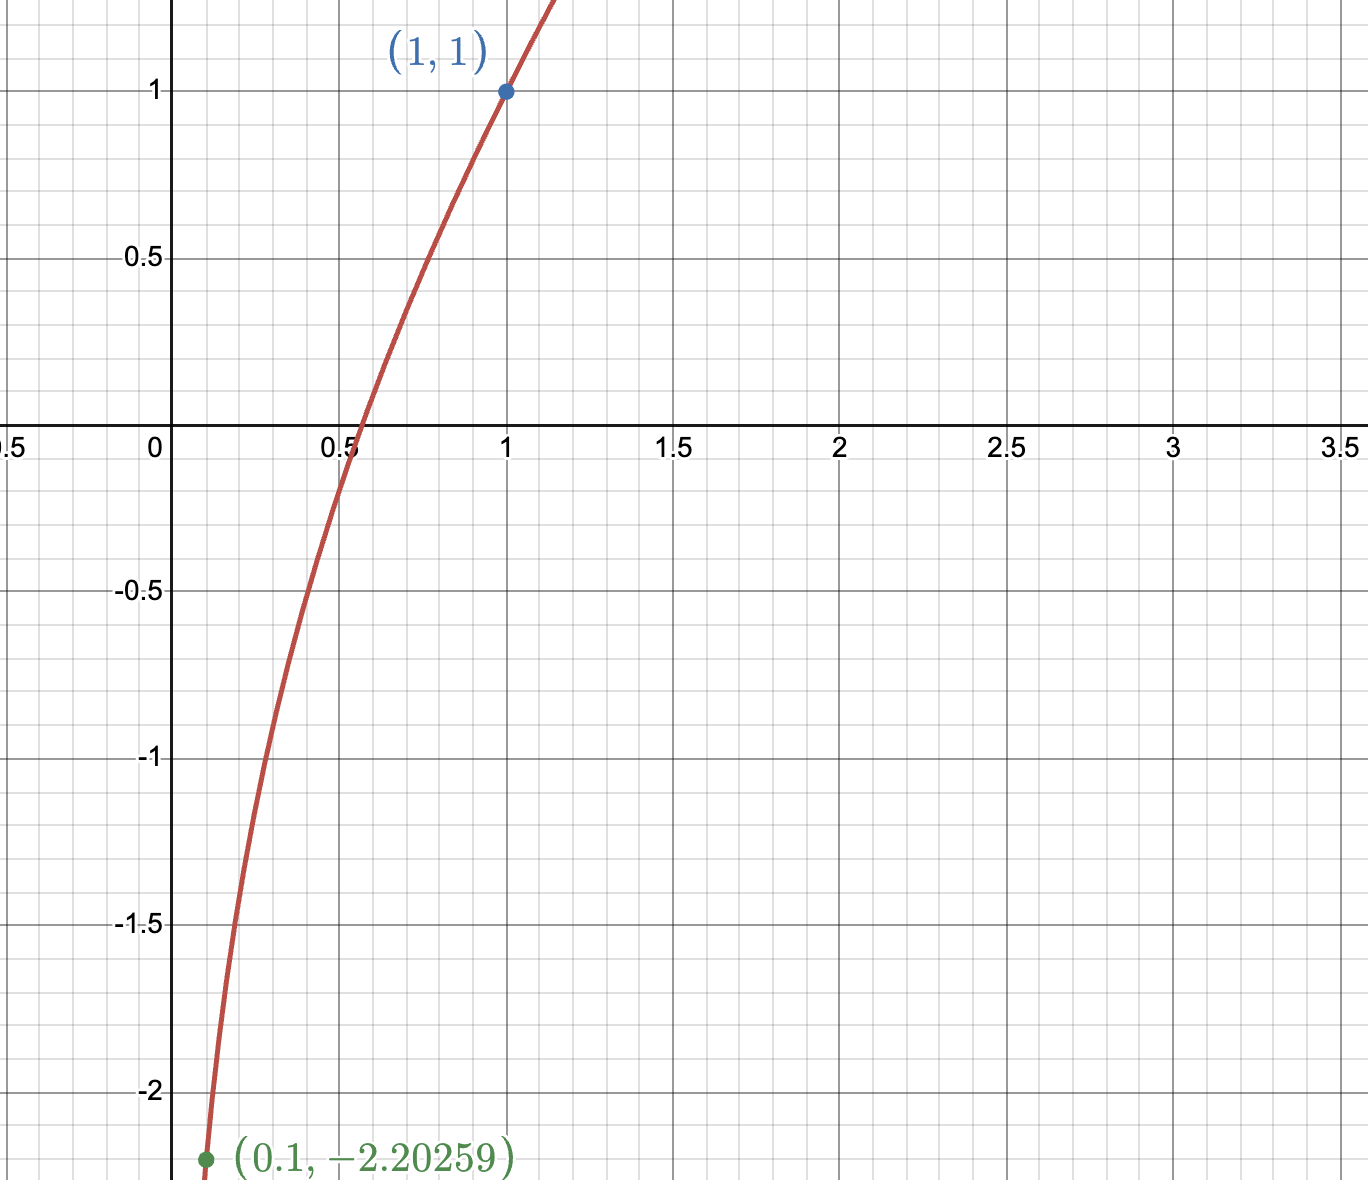
\includegraphics[width=10cm]{graph.png}
    \end{center}
    \item Let us apply the mentioned methods. Here is the driver code I use throughout this process.
  \begin{lstlisting}[language=Matlab]
function find_roots()
  f = @(x) x + log(x);
  df = @(x) 1 + 1/x;
  % Convergence criterion
  tol = 1e-10;
  max_iter = 100;
  % 1. Bisection Method
  [x_bisect, iter_bisect] = bisection(f, 0.5, 0.6, tol);
  % 2. Fixed Point Iteration
  g = @(x) exp(-x);
  [x_fixed, iter_fixed] = fixed_point(g, 0.5, tol, max_iter);
  % 3. Newton's Method
  [x_newton, iter_newton] = newton(f, df, 0.5, tol, max_iter);
  % 4. Secant Method
  [x_secant, iter_secant] = secant(f, 0.5, 0.6, tol, max_iter);
  fprintf('Method      | Root          | Iterations\n');
  fprintf('Bisection   | %.10f | %d\n', x_bisect, iter_bisect);
  fprintf('Fixed Point | %.10f | %d\n', x_fixed, iter_fixed);
  fprintf('Newton      | %.10f | %d\n', x_newton, iter_newton);
  fprintf('Secant      | %.10f | %d\n', x_secant, iter_secant);
end
  \end{lstlisting}
  \end{enumerate}
  
  \begin{enumerate}[i.]
    \item For the Bisection Method, the interval $[0.5, 0.6]$ is valid because 
    $f(0.5) * f(0.6) < 0$, and so since the endpoints are opposite signs, by the IVT, the function attains 
    all values in between, and so there must be at least one root in the interval.
    \begin{lstlisting}[language=Matlab]
function [x, iter] = bisection(f, a, b, tol)
  iter = 0;
  while (b - a) / 2 > tol
      p = (a + b) / 2;
      if f(p) == 0
          break;
      elseif f(a) * f(p) < 0
          b = p;
      else
          a = p;
      end
      iter = iter + 1;
      fprintf('Bisection Method Iteration %d: x = %.10f\n', iter, p);
  end
  x = (a + b) / 2;
  fprintf('Error: %.10f\n', abs(p - fzero(f, [0.5, 0.6])))
end
    \end{lstlisting} 
    \begin{center}
      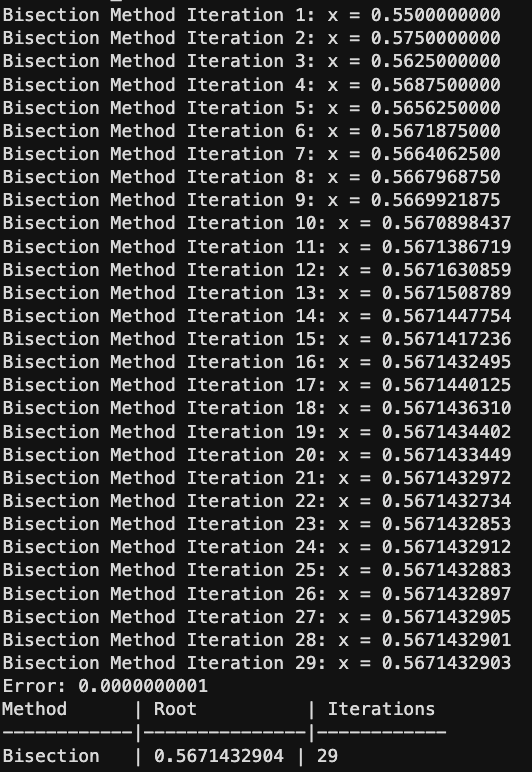
\includegraphics[width=8cm]{bisection-progress.png}
    \end{center}
    The expected number of iterations using Bisection Method is
    \[\text{ceil}\left( \frac{\log(b-a) - \log(2 * \text{atol})}{\log 2}\right) = \text{ceil}(28.89) = 29\]
    and so our results match theoretical expectations.

\item For Fixed Point Iteration, define $f(x) = x + \ln x$. We want to cleverly choose $g(x)$ 
so it's easy to find $x^*$ such that $f(x^*) = 0$. 
Consider $g(x) = -\exp(x)$
\[g(x) = \exp(-x) \implies x^* = \exp(-x^*) \implies \ln(x^*) = -x^*\]
\[\implies x^* + \ln(x^*) = 0 \implies f(x^*) = 0\]
\begin{lstlisting}[language=Matlab]
function [x, iter] = fixed_point(g, x0, tol, max_iter)
  x = x0;
  iter = 0;
  fprintf('Fixed Point Iteration:\n');
  fprintf('Iteration 0: x = %.10f\n', x);
  while iter < max_iter
      x_new = g(x);
      if abs(x_new - x) < tol
          break;
      end
      x = x_new;
      iter = iter + 1;
      fprintf('Iteration %d: x = %.10f\n', iter, x);
  end
  fprintf('Error: %.10f\n', abs(x - fzero(@(x) x - exp(-x), [0.5, 0.6])))
end
\end{lstlisting}
\begin{center}
  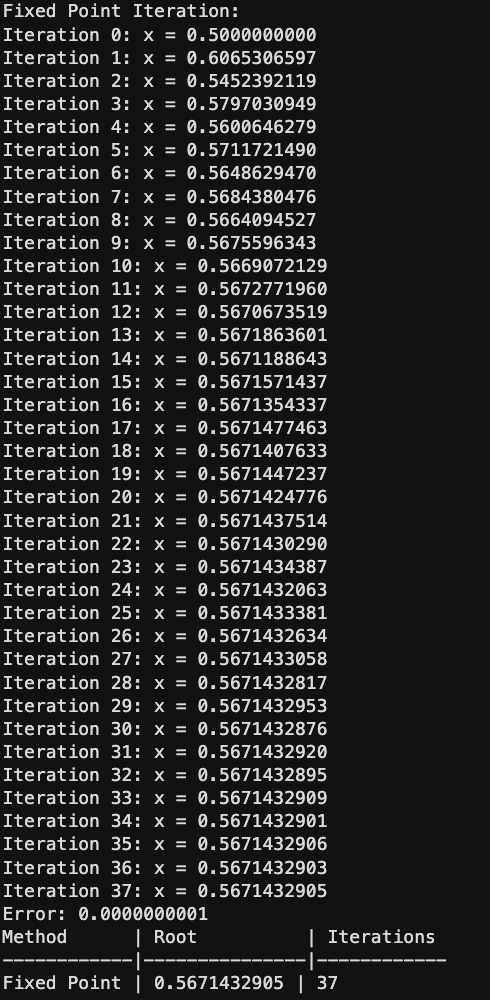
\includegraphics[width=8cm]{fixed-progress.png}
\end{center}
Note that $g(x) = \exp(-x) \implies g'(x) = -\exp(-x)$. Looking at the graph, $|g'(x)| < 0.65 \ \forall \ x \in [0.5, 0.6]$. 
Therefore, since $\rho < 1$, the uniqueness and convergence proofs which leverage First Order Taylor Series expansions provided in class 
are applicable, and our results match the theoretical expectations of linear convergence since the algorithm converges 
in $37$ iterations.
\item Newton's Method with $x_0 = 0.5$
\begin{lstlisting}[language=Matlab]
function [x, iter] = newton(f, df, x0, tol, max_iter)
  x = x0;
  iter = 0;
  while iter < max_iter
      x_new = x - f(x) / df(x);
      if abs(x_new - x) < tol
          break;
      end
      x = x_new;
      iter = iter + 1;
      fprintf('Newton Iteration %d: x = %.10f\n', iter, x);
  end
  fprintf('Error: %.10f\n', abs(x - fzero(f, [0.5, 0.6])))
end
\end{lstlisting}
\begin{center}
  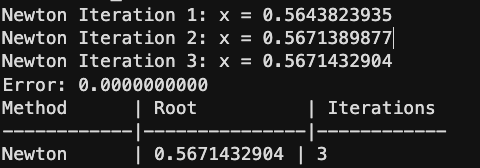
\includegraphics[width=8cm]{newton-progress.png}
\end{center}
Since we started in the neighborhood of the root and Newton's Method has 
quadratic convergence, we were able to converge to the root in only $3$ iterations, which is much faster than
the $37$ iterations required for fixed point iteration, which is expected because fixed point iteration 
has linear convergence. 
\item Finally, the Secant Method with $x_0 = 0.5$ and $x_1 = 0.6$
\begin{lstlisting}
function [x, iter] = secant(f, x0, x1, tol, max_iter)
  iter = 0;
  while iter < max_iter
      x_new = x1 - f(x1) * (x1 - x0) / (f(x1) - f(x0));
      if abs(x_new - x1) < tol
          break;
      end
      x0 = x1;
      x1 = x_new;
      iter = iter + 1;
      fprintf('Iteration %d: x = %.10f\n', iter, x1);
  end
  x = x1;
  fprintf('Error: %.10f\n', abs(x - fzero(f, [0.5, 0.6])))
end
\end{lstlisting}
\begin{center}
  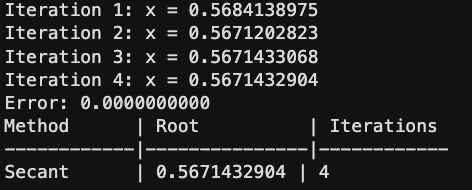
\includegraphics[width=8cm]{secant-progress.png}
\end{center}
The Secant Method converges in $4$ iterations. Recall that the Secant Method is guaranteed 
superlinear convergence, so this result makes sense that it's slower than Newton's Method which has 
quadratic convergence and faster than Fixed Point Iteration which has linear convergence. 
\end{enumerate}
\end{proof}

\end{document}

